Nogle gange kan vi ikke benytte integralregningens hovedsætning til at bestemme værdien af et integral, da vi ikke er i stand til at finde en stamfunktion.
I det tilfælde er det praktisk at kunne bestemme værdien af integralet numerisk.
Vi præsenterer her kort Simpsons metode, der tilnærmer arealet under grafen for en kontinuert funktion ved hjælp af parabler.\footnote{Afsnittet er baseret på \cite{Bartle2010}, s. 238-239.}

\subsection{Simpsons metode}%
\label{sub:Simpsons metode}

Før vi kan angive en formel for Simpsons metode, vil vi først kigge på arealet under grafen for et andengradspolynomium, der er bestemt af tre givne punkter.

\begin{example}[label=exa:andengrad]{Areal under grafen for andengradspolynomium bestemt af tre punkter}{}
  Betragt andengradspolynomiet, der går gennem de tre punkter
  \[
  (-h, y_0), (0, y_1) \text{ og } (h, y_2).
  \] 
  Andengradspolynomiet må være af formen $p(x)=ax^2+bx+c$.
  Siden $p(0)=y_1$, så har vi $c=y_1$.
Vi får da ligningssystemet
\begin{equation*}
\begin{split}
  a (-h)^2 -bh + y_1&=y_0 \\
  a h^2 + bh + y_1&=y_2.
\end{split}
\end{equation*}
  Løser vi ligningssystemet, får vi 
  \[
  a=\frac{y_0-y_1+\frac{y_2-y_0}{2}}{h^2} \text{ og }b=\frac{y_2-y_0}{2h}. 
  \] 
  Arealet under grafen fra $-h$ til $h$ må være
  \begin{equation*}
  \begin{split}
    \int_{-h}^{h} (ax^2+bx+c) \,dx &= 2 \cdot \int_{0}^{h} \left(ax^2+c\right)  \,dx \\
    &=2 \cdot \left[\frac{x^3}{3} a + cx\right]_0^h \\
    &=2 \cdot \left(\frac{h^3}{3}a + ch\right) \\
    &=\frac{h}{3}\left(2ah^2+6c\right) \\
    &=\frac{h}{3} \left(2 \cdot \left(y_0-y_1 + \frac{y_2-y_0}{2}\right) + 6y_1\right) \\
    &=\frac{h}{3} \left(y_0+4y_1+y_2\right).
  \end{split}
  \end{equation*}
 Arealet under grafen for det givne andengradspolynomium fra $-h$ til $h$ er altså $\frac{h}{3} \left(y_0 + 4y_1 + y_2\right) $.
\end{example}

Ideen i Simpsons metode er så, at vi kan bruge dette udtryk til at bestemme arealet under hvert af andengradspolynomierne vi approksimerer med, da $y$-værdierne og dermed arealet ikke ændres ved en horisontal forskydning.
En intuitiv måde at forstå formlen for Simpsons metode er nemlig, at vi vandret forskyder midtpunktet af hver parabel til $x=0$, hvor vi så kan benytte den udledte formel fra eksempel \ref{exa:andengrad}.

For en kontinuert funktion $f:[a;b]\to \mathbb{R}$ deler vi intervallet $[a;b]$ op i $n$ delintervaller, der hver har længden $h=\frac{b-a}{n}$.
På hvert dobbelt delinterval
\[
[a;a+2h], [a+2h;a+4h], \ldots , [b-2h;b],
\] 
kan vi så tilnærme os en værdi for arealet under grafen med en parabel.
Vi får da
\begin{equation*}
\begin{split}
  \int_{a}^{b} f &\approx \frac{h}{3} \left(y_0 + 4y_1 +y_2\right) + \frac{h}{3} \left(y_2 + 4y_3 +y_4\right) + \cdots \frac{h}{3} \left(y_{n-2} + 4y_{n-1} +y_n\right)\\
  &=\frac{h}{3} \left(y_0 + 4y_1 + 2y_2 + 4y_3 + 2y_4 + \cdots +2y_{n-2} + 4 y_{n-1} + y_n\right),
\end{split}
\end{equation*}
hvor $y_i=f(a+ih)$ for $i=0,\ldots , n$. 
Dette fører til den næste definition.

\begin{definition}[label=def:Simpson]{$n$'te Simpson-approksimation}{}
  Antag en reel funktion $f$ er kontinuert på $[a;b]$, $n \in \mathbb{N}$ er et lige tal, og lad $h_n=\frac{b-a}{n}$.
  Så er den $n$'te Simpson-approksimation defineret ved
  \begin{equation*}
  \begin{split}
    S_n(f)=&\frac{h_n}{3} (f(a) + 4f(a+h_n) + 2f(a+2h_n) + 4f(a+3h_n) \\
    &+ 2f(a+4h_n) + \cdots + 2f(b-2h_n) + 4f(b-h_n)+ f(b)).
  \end{split}
  \end{equation*}
\end{definition}

Det er åbenlyst, at jo større $n$ er, desto bedre er approksimationen. 
Som eksempel på en Simpson-approksimation bestemmer vi sandsynligheden for et udfald inden for to spredninger af middelværdien for standardnormalfordelingen.

\begin{figure}[H]
\begin{center}
  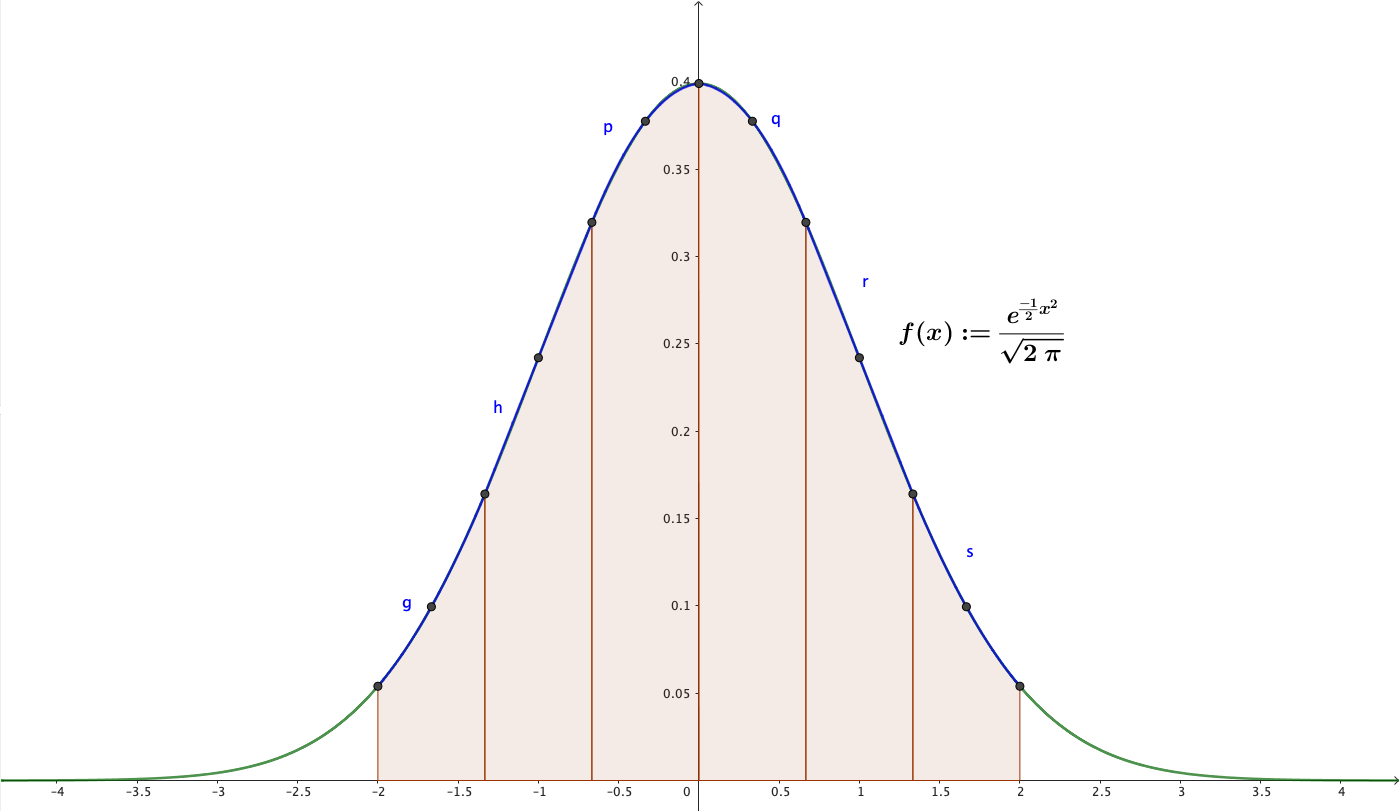
\includegraphics[width=\textwidth]{fig/standardnormalfordeling.png}
\end{center}
  \caption{Ved Simpsons metode beregnes summen af arealerne under hver parabel (de blå)}
\label{fig:standardnormalfordeling}
\end{figure}
 

\begin{example}[label=exa:standardnormalfordeling]{Sandsynlighed i standardnormalfordelingen }{}
  Tæthedsfunktionen for standardnormalfordelingen er givet ved
  \[
  f(x)=\frac{e^{-\frac{x^2}{2}} }{\sqrt{2 \pi } }.
  \] 
Vi vil finde en tilnærmet værdi for sandsynligheden for et udfald inden for to spredninger af middelværdien.
  Med andre ord vil vi approksimere sandsynligheden $P(-2 \leq X \leq 2) = \int_{-2}^{2} f$.
  Dette gør vi med den 12'te Simpson-approksimation.
  Så får vi $h_{12}$ til
  \[
  h_{12}=\frac{2-(-2)}{12}=\frac{1}{3}.
  \] 
  Vi udregner Simpson-approksimationen med CAS, hvilket ses i \cref{fig:CAS}.
  \begin{equation*}
  \begin{split}
    \int_{-2}^{2} \left(\frac{e^{-\frac{x^2}{2}} }{\sqrt{2 \pi } }\right)\,dx  \approx& \,S _{12}(f)\\
    =&\frac{1}{3^2} \Biggl(f(-2) + 4f\left(-\frac{5}{3}\right) + 2f\left(-\frac{4}{3}\right) + 4f(-1) + 2f\left(-\frac{2}{3}\right) + 4 f\left(-\frac{1}{3}\right) \\ 
    &+ 2 f(0) + 4 \left(\frac{1}{3}\right) + 2 \left(\frac{2}{3}\right) + 4 \left(1\right)  + 2f\left(\frac{4}{3}\right) + 4f\left(\frac{5}{3}\right)+ f(2)\Biggl)\\
    \approx& \,0,9544830603.
  \end{split}
  \end{equation*}
  Dette er utroligt tæt på den 'rigtige' værdi til ti betydende cifre, som er $0,9544997361$.
  \begin{figure}[H]
  \begin{center}
    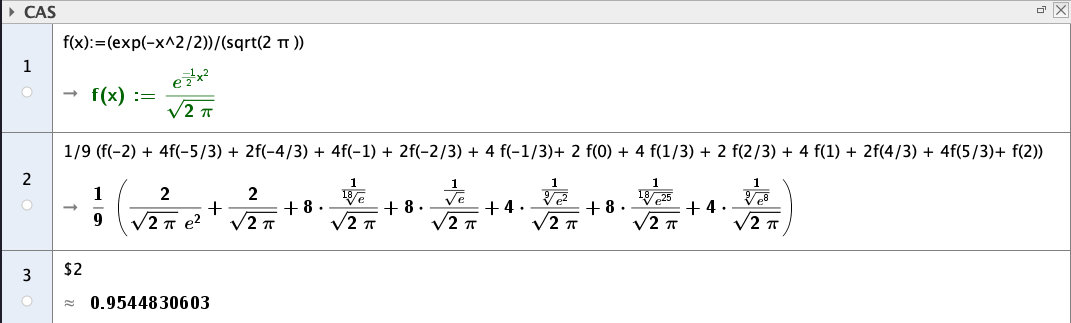
\includegraphics[width=\textwidth]{fig/CAS10deci.png}
  \end{center}
  \caption{Den 12'te Simpson-approksimation udregnet med CAS}
  \label{fig:CAS}
  \end{figure}
\end{example}
 


